% Part of the layout information as well as title, logo are defined in the style file, e.g. beamerthemeOregon.sty
\documentclass{beamer}
\mode<presentation>
{
  \usetheme{NCAR}
  \setbeamercovered{transparent}
}
\usepackage{times}


\usepackage{amsmath,amssymb}
\usepackage[english]{babel}
\usepackage[latin1]{inputenc}
\usepackage[orientation=landscape,size=a0,scale=1,debug]{beamerposter}   % scale only seems to apply to text
\usepackage{framed, color} % to produce boxes, e.g. for conclusions
\definecolor{shadecolor}{RGB}{169,202,222}

\usepackage{ragged2e} % to use \justifying

\usepackage{natbib}
 \def\newblock{\hskip .11em plus .33em minus .07em}

\usepackage[absolute,overlay]{textpos}
\TPGrid[0cm,0cm]{100}{100} % choose \TPHorizModule and \TPVertModule so as to give a grid of 100 intervals across and 100 intervals down
\TPMargin{1cm}

\textblockorigin{0mm}{90mm} %sets the origin of the page - the 0,0 point of the coordinate system

\usepackage{tikz}
% \usetikzlibrary{snakes}

\title[]{{The Development of Quantitative Hydrologic Storylines to Understand Uncertainty in Climate}}

\makeatletter
\def\beamer@andinst{\\[0.1em]}
\makeatother

\author[]{Ethan Gutmann\inst{1}, \and Martyn Clark\inst{1}, \and Andy Wood\inst{1}, \and Joseph Hamman\inst{1}, \and Julie Vano\inst{1}, \and Levi Brekke\inst{1}, \and Ken Nowak\inst{2}, \and Jeffrey Arnold\inst{3}}
\institute[]{\inst{1}National Center for Atmospheric Research, Research Applications Lab, Boulder, United States \and \inst{2}Bureau of Reclamation, Denver, United States \and \inst{3}US Army Corps of Engineers, Climate Preparedness and Resilience Programs, United States}

\date{April 2017}

\newcommand{\degC}{$^{\circ}$C}

\setbeamertemplate{caption}{\insertcaptionname~\insertcaptionnumber:
\insertcaption}

\begin{document}

\begin{frame}{}
 \vspace{2cm}

 \begin{columns}

  %%% FIRST COLUMN

  \begin{column}{.3333\paperwidth} % if all columns have the same width, it's enough to declare that width once

   \begin{textblock}{\textwidth \TPHorizModule}(0,0)
    \begin{block}{1. Introduction}

     \begin{itemize}
      \justifying

      \item Future climate projections are inherently uncertain, and quantifying and managing this uncertainty is one of the key tasks in any climate application.
      \item Previous research assessing climate change impacts on hydrologic systems has revealed a clear need to better understand how uncertainty in hydrologic projections propagates through traditional modeling chains.
      \item This uncertainty stems from chaotic variability in the climate system as well as uncertainty due to the methods we use (either from lack of understanding of the system or intentional simplifications in our models).
      \item We are particularly interested in the uncertainty that comes from methodological choices related to emissions scenarios, climate models, downscaling models, and hydrology models (see Figure \ref{fig:storylines}).

     \end{itemize}

    \end{block}
   \end{textblock}


   \begin{textblock}{\textwidth \TPHorizModule}(0,18)
    \begin{block}{2. Hydrologic Storylines}

     \begin{itemize}
      \justifying

      \item We aim to develop a smaller set of representative hydrologic projections or ``storylines'' while specifically addressing the leading contributors of uncertainty.
      \item The first step is to characterize the uncertainties in the ``full'' ensemble to understand where and how much each component of the model chain contributes to the full ensemble's uncertainty.
      \item The second phase of the project will focus on reducing uncertainties by refining methodologies.
      \item Finally, distinct hydrologic storylines will be developed using data-driven and bottom-up methods.

     \end{itemize}

     \begin{figure}
      \center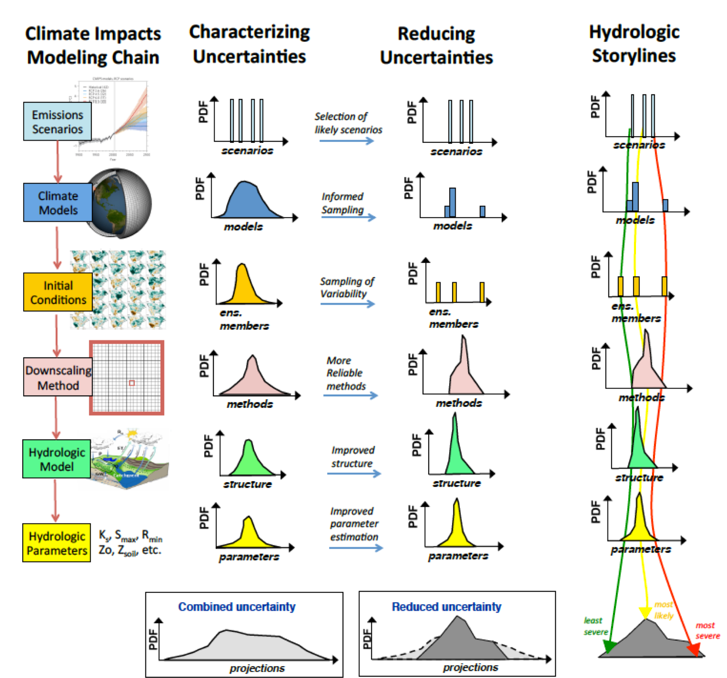
\includegraphics[width=\linewidth]{figures/storylines_diag.png}
      \caption{Schematic on approaches to explicitly characterize and reduce the myriad uncertainties in assessments of the hydrologic impacts of climate change and the development of representative quantitative hydrologic storylines for specific applications. Caption and figure from \citep{Clark_2016}.
       \label{fig:storylines}}
     \end{figure}

    \end{block}
   \end{textblock}


   %%% SECOND COLUMN

   \begin{textblock}{\textwidth \TPHorizModule}(33.333,0)
    \begin{block}{3. Downscaling}

     \begin{tikzpicture}[]

      % draw horizontal line
      \draw (0,0) -- (33.333,0);
      %   \draw[snake] (2,0) -- (4,0);
      %   \draw (4,0) -- (5,0);
      %   \draw[snake] (5,0) -- (7,0);

      % draw vertical lines
      \foreach \x in {0,5,12,22,33.333}
      \draw[->,line width=3pt] (\x cm,0) -- (1+\x cm,0);

      % draw nodes
      \draw (0,0) node[below=3pt] {Raw GCM};
      \draw (5,0) node[below=3pt] {BCSD};
      \draw (12,0) node[below=3pt] {Multivariate Regression};
      \draw (22,0) node[below=3pt] {Reduced Physics RCM};
      \draw (31,0) node[below=3pt] {High-res RCM};

      \node[above,font=\large\bfseries] at (current bounding box.north) {The complexity continuum of climate downscaling methodologies};

     \end{tikzpicture}

     \begin{itemize}
      \justifying

      \item A wide array of downscaling and bias correction methodologies have been proposed.
      \item Not all downscaling methods are created equal. Some methods should not be used for hydrologic modeling. See \citet{Gutmann_2014}.
      \item We are developing the Generalized Analog Regression Downscaling (GARD) tool to provide a simple statistical downscaling method relying on regressions and statistical transformations from various inputs (e.g. precipitation, humidity, wind, PCA, etc.) to various outputs (e.g. precipitation, temperature, etc.). See http://gard.readthedocs.io/.
      \item Simple / existing downscaling methods (e.g. BCSD) are being compared to progressively more complex methods like GARD, ICAR, and WRF to better understand how methodological complexity is related to fidelity and sensitivity.

     \end{itemize}

     \begin{figure}
      \center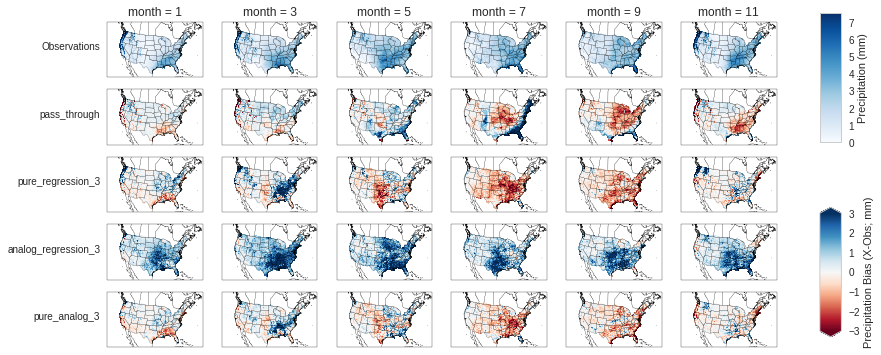
\includegraphics[width=\linewidth]{figures/downscaling.png}
      \caption{Comparison of precipitation predicted using 4 different downscaling approaches using GARD. Row1: Gridded (1/8deg) observed precipitation from Maurer et al (2001), Row 2: 50-km WRF precipitation interpolated to observations grid, Row 3-5: precipitation derived from multi-variate linear regression, analog, and analog regression techniques using predictor variables of precipitation, U/V winds, and SLP.}
      \label{fig:downscaling}
     \end{figure}

    \end{block}

   \end{textblock}



   \begin{textblock}{\textwidth \TPHorizModule}(33.333,45)
    \begin{block}{4. Hydrologic Modeling}

     \begin{figure}
      \center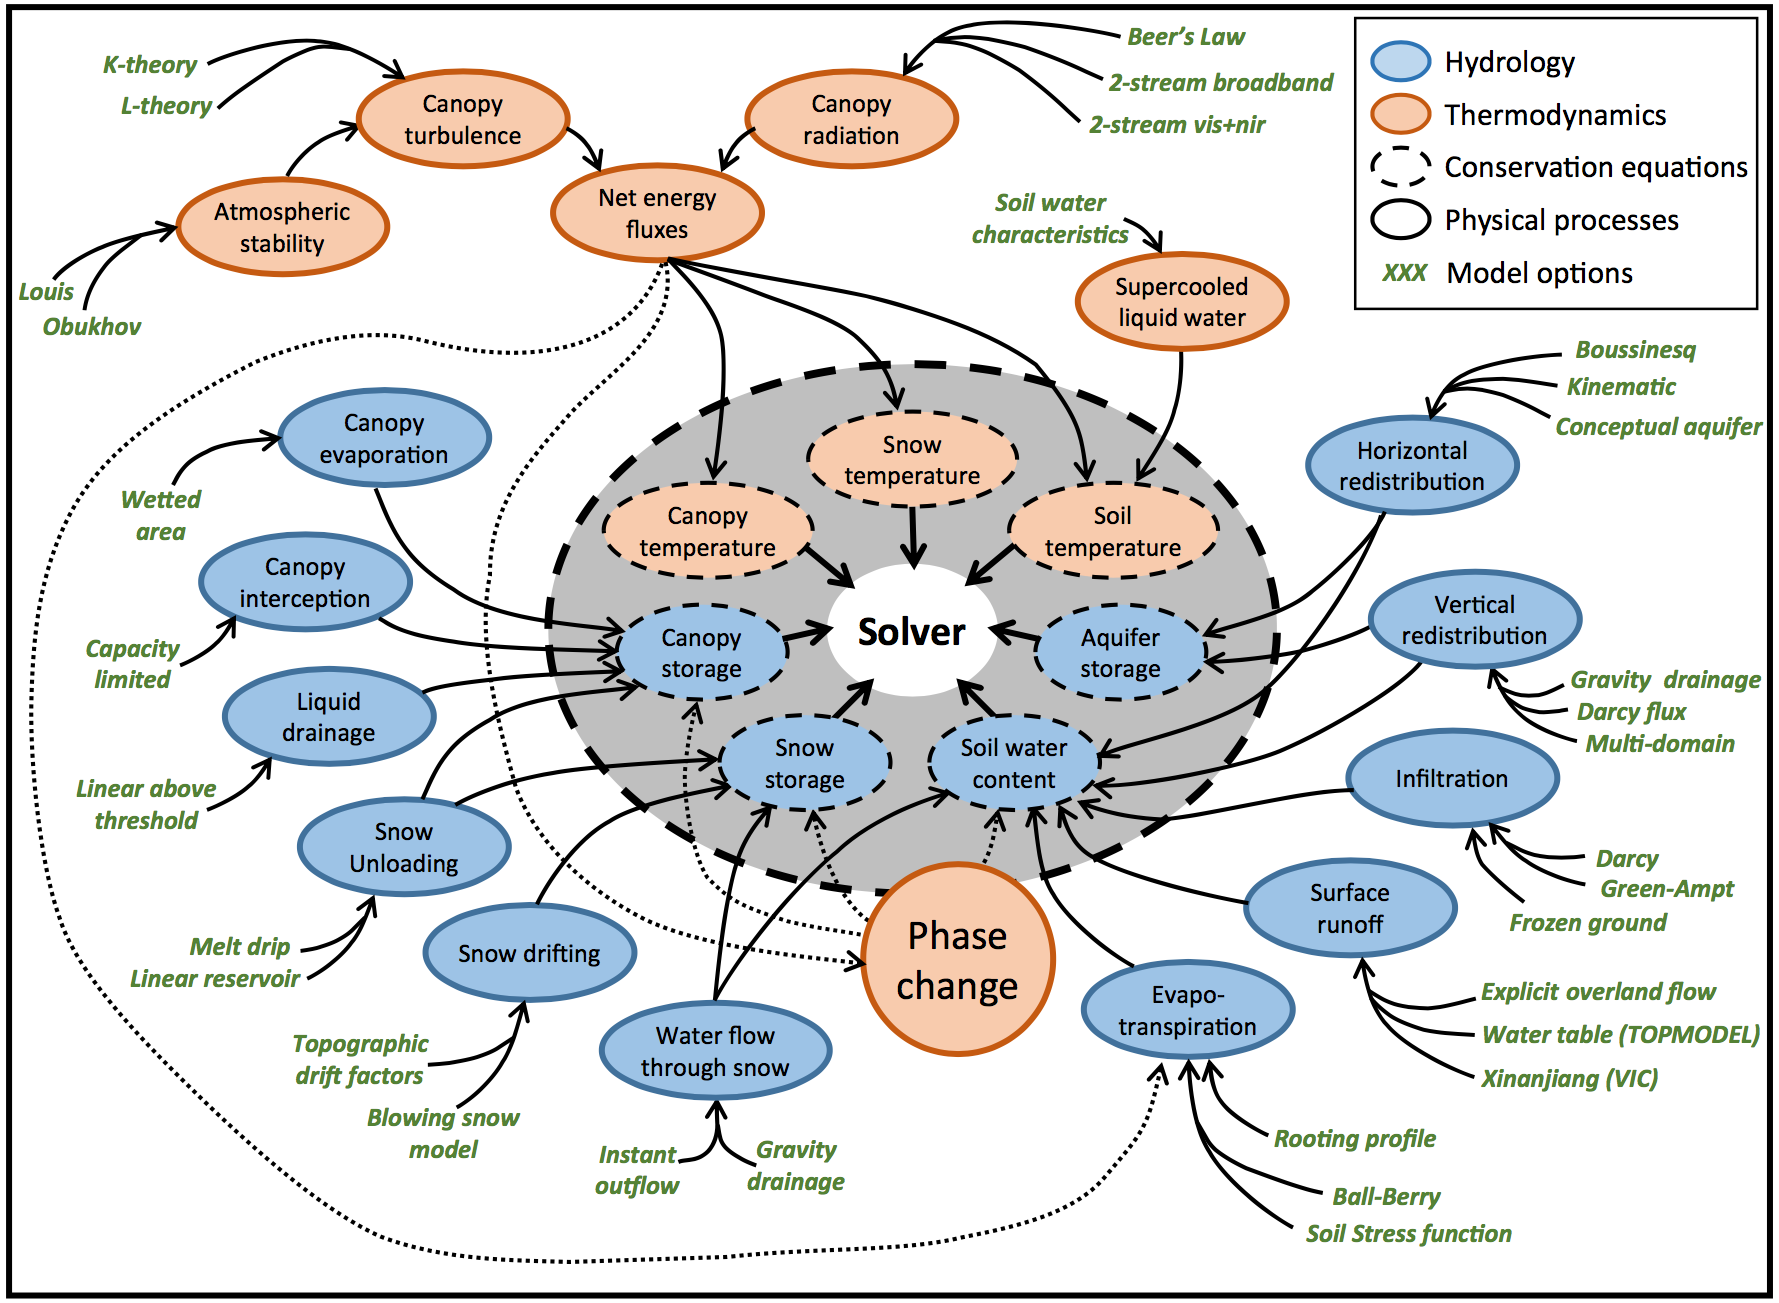
\includegraphics[width=0.6\linewidth]{figures/summa.png}
      \caption{Conceptual diagram illustrating the SUMMA framework for supporting multiple alternative model options for a range of physical processes, integrated as part of a common numerical solver. Figure and caption adapted from \citet{Clark_2015}.}
      \label{fig:summa}
     \end{figure}

     \begin{itemize}
      \justifying
      \item Traditional hydrologic climate impacts studies have not looked at how hydrologic model structure or model parameters influence the inferences derived from the modeling activity.
      \item We will use the Structure for Unifying Multiple Modeling Alternatives (SUMMA) model \citep{Clark_2015} to generate large a series of different modeling approaches using the same structural core (see Figure \ref{fig:summa}). Using SUMMA allows for the controlled and systematic analysis of modeling options and complexities.
      \item Model parameters will be derived using the Multi-scale Parameter Regionalization (MPR) method of \citet{Samaniego_2010}. Using MPR allows for the generation of ensembles of parameters, derived from calibrations performed using an array of objective functions.
     \end{itemize}

    \end{block}
   \end{textblock}


   %%% THIRD COLUMN

   \begin{textblock}{\textwidth \TPHorizModule}(66.667,0)
    \begin{block}{5. Outlook: Production of large ensembles of hydrologic projections}

     \begin{itemize}
      \justifying
      \item We are developing a large ensemble of hydrologic projections over the CONUS domain.
      \item Our controlled evaluation of both the climate forcing and hydrologic modeling will allow for increased understanding of uncertainty derived from each component of the climate impacts modeling chain.
     \end{itemize}

     \begin{figure}
      \center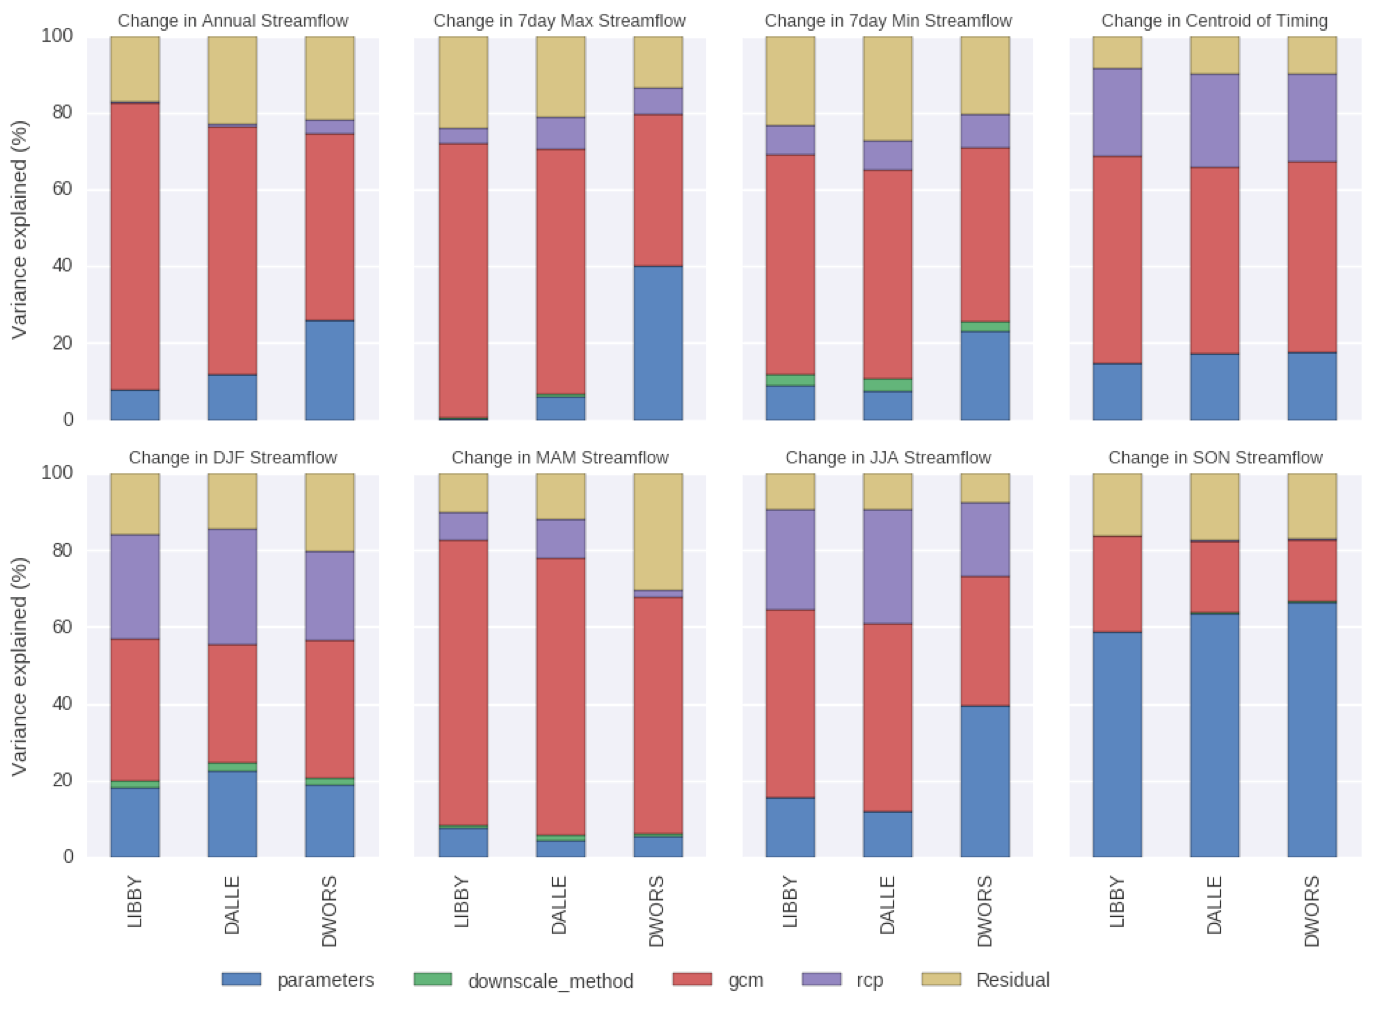
\includegraphics[width=0.7\linewidth]{figures/anova.png}
      \caption{Example of an ANOVA analysis performed using a combination of existing data from the University of Washington RMJOC dataset and the NCAR BCSD dataset. The total dataset includes 2 RCPs, 10 GCMs, 2 downscaling Methods, 1 hydrologic model (VIC), and 4 hydrologic model parameter sets. Each subplot represents a different analysis metric. Each column is a different watershed in the Columbia River Basin.
       \label{fig:anova}}
     \end{figure}

     \begin{itemize}
      \justifying
      \item Figure \ref{fig:anova} provides an example, using existing datasets, of how uncertainty (variance) can be partitioned.
      \item Key point: the variance explained by each variable is substantially different between different analysis metrics.
     \end{itemize}

    \end{block}
   \end{textblock}

   \begin{textblock}{\textwidth \TPHorizModule}(66.667,45)


    \begin{block}{6. Conclusions}

     \begin{shaded}

      \begin{itemize}         \vspace{1cm}
       \justifying
       \item Hydrologic climate projections have uncertainty from the climate forcing (emissions scenarios, climate models, initial conditions) and from the hydrologic modeling application (model structure and parameters). We are systematically characterizing these uncertainties. \vspace{1cm}
       \item We are developing new climate downscaling tools (GARD, ICAR) to fill in the complexity continuum. These tools will facilitate new analysis approaches that target the relationship between complexity, fidelity, and sensitivity. \vspace{1cm}
       \item New data-driven and bottom-up sampling methods are being developed to enable the selection of smaller sets of representative hydrologic projections (storylines) while addressing the leading contributors of uncertainty. \vspace{1cm}

      \end{itemize}

     \end{shaded}



    \end{block}
   \end{textblock}

   \vspace{2cm}

   \begin{textblock}{\textwidth \TPHorizModule}(66.667,69)
    \begin{block}{References}


     \justifying
     \bibliographystyle{apalike}

     \small\bibliography{library} % this command does not accept white spaces in the path, I made a symbolic link to the *.bib generated in Mendeley and stored in Google Drive

    \end{block}
   \end{textblock}


  \end{column}
 \end{columns}
\end{frame}

\end{document}
